\section{Method: Action Research - Drools in MPS}\label{section:Method_action_research}

Even though Drools is a relatively small DSL, we did not feel the need to implement all of the functionality to answer our questions.

\subsection{Really Simple Rules Language}
As we were new to DSL design and MPS, we First would create a very simple approximation of the Drools language with which to create our first projections.
We called this language "Really Simple Rules" (RSR).

\paragraph{File} RSR, Like Drools itself, has a File as it's root node.
The file only contains Facts and Rules.

\paragraph{Fact and FactProperty} In Drools a fact represents a Java Bean with its subsequent properties which can also be types with their own properties.
In RSR we limited properties to only allow boolean values.
This decision was based on the fact selection is a predicate and thus can only return a boolean.
By only having booleans we also limit the operations on the property.

\paragraph{Rule} For the Rules Concept, we decided to only simulate the Left Hand Side, or "When" conditions", of a Drools Rule.
We believed this would be enough to provide us with interesting projections, and did not want to over complicate this first approach.
An RSR Rule consists of a collection of conditions. 
Should all those conditions return true then the rule is selected.

\paragraph{Condition} A condition operates on one or more FactSelectors.
There are four condition type Exists, Not, And, and Or.
Exists and Not are unary conditions and evaluate one FactSelector.
And and Or evaluate two Fact Selectors.

\paragraph{FactSelector} a FactSelector consists of a reference to a Fact and a collection of Predicates.
If the Fact exists and all the predicates evaluate to true then the fact selector evaluates to true.

\paragraph{Predicate} the predicate is an operation on a fact property, to which the concept has a reference.
As the fact property represents a boolean value, then the only predicate operations are ``Is'' and ``Not''.

Figure \ref{fig:RSRDiagram} shows the Concept hierarch for this very simple implementation.

\begin{figure}[h]
    \centering
    \fbox{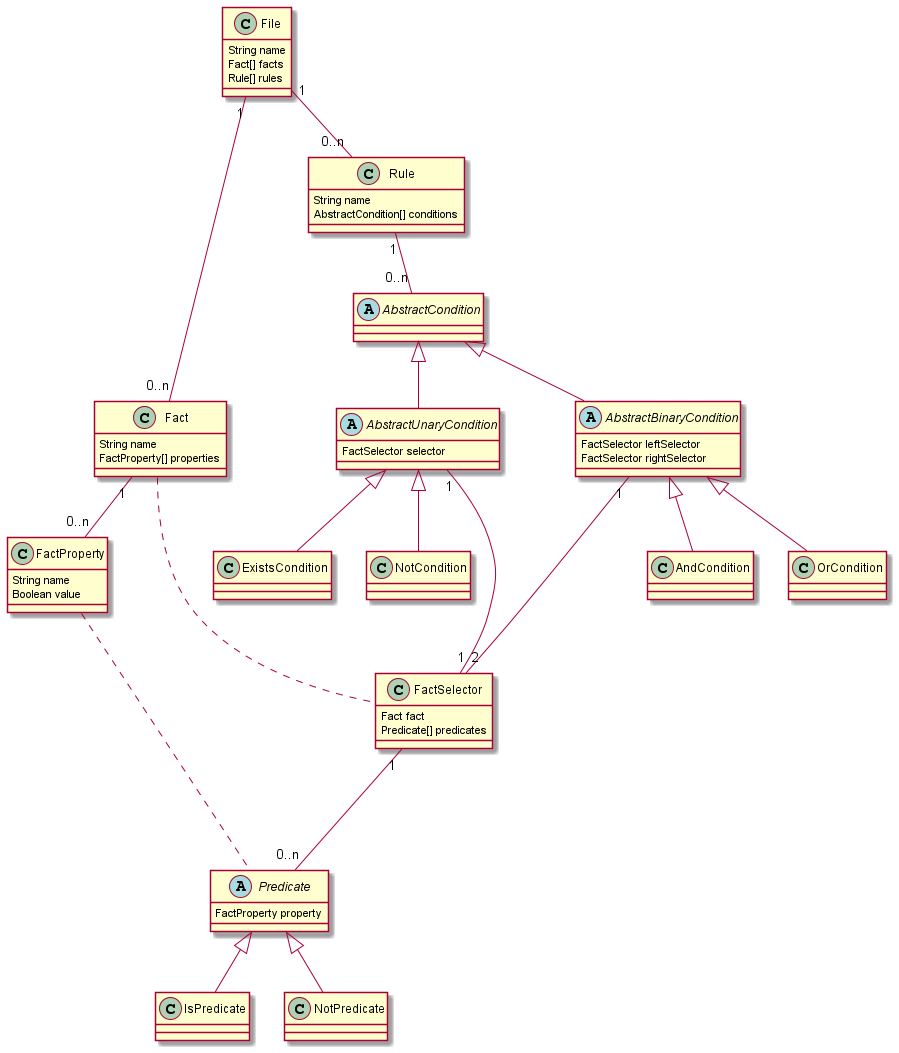
\includegraphics[width=0.95\textwidth]{Sections/images/ReallySimpleRuleLanguage.png}}
    \caption{RSR Concept Hierarchy}
    \label{fig:RSRDiagram}
\end{figure}

This design was then realised in MPS.
As the aim is to attempt different projections we did not initially optimise for editing.
The structure is as show in figure \ref{fig:RSRStructure} and the editors including those shown in figure \ref{fig:RSREditors}.

\begin{figure}
    \centering
    \begin{minipage}{0.30\textwidth}
        \centering
        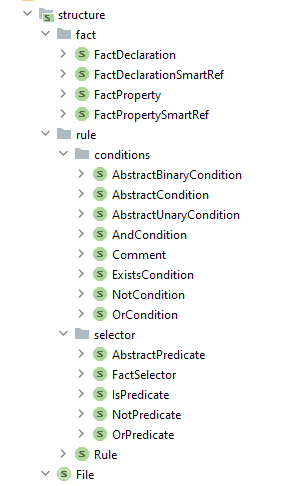
\includegraphics[width=0.9\textwidth]{Sections/images/RSRStructrure.png}
        \caption{RSR}
        \label{fig:RSRStructure}
    \end{minipage}\hfill
    \begin{minipage}{0.70\textwidth}
        \centering
        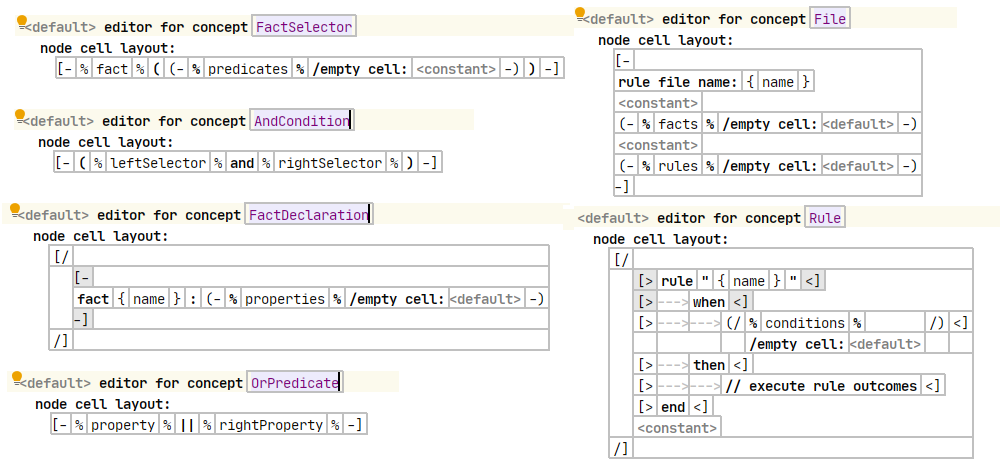
\includegraphics[width=0.9\textwidth]{Sections/images/RSREditors.png} 
        \caption{Editors}
        \label{fig:RSREditors}
    \end{minipage}
\end{figure}

Part of the research question is using projections to reason about large files.
In order to answer this we needed to simulate a large file.
To do this we had to enter a large number of rules.
As this becomes tedious we added a number of editing aids including substitute menus to speed up the entry of conditions, as shown in figure \ref{fig:RSRSubstituteMenu}.
This image, shows that before I had to select an ExistsCondition concept, and thereafter select the Fact for the condition.
After adding the substitute menu, I could immediate select the Fact I wanted and it would then automatically be wrapped with an ExistsCondition node. I could immediatly select the Fact and the 

\begin{figure}[h]
    \centering
    \fbox{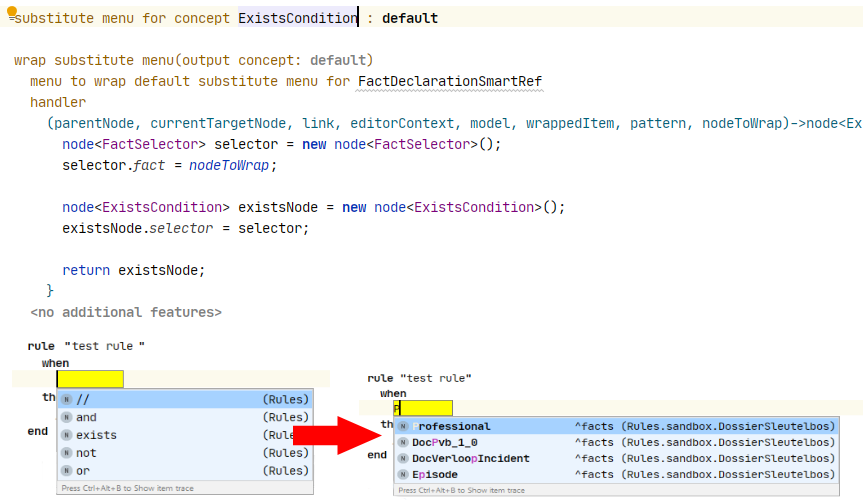
\includegraphics[width=0.95\textwidth]{Sections/images/RSRSubstituteMenu.png}}
    \caption{RSR Substitute Menu}
    \label{fig:RSRSubstituteMenu}
\end{figure}

We also added some intentions to invert incorrectly added conditions.

Finally, we added a constraint to scope the fact properties in predicates to the Fact chosen in the FactSelector.
This made it much easier to select properties in the predicates as indicated in figure \ref{fig:RSRConstraint}.
In the figure you can see that before the scoping constraint it showed a list with dozens of potential FactProperties, that represented all the FactProperties in the Model.
After the constraint is added it only shows the two properties associates with the Fact from the FactSelector.

\begin{figure}[h]
    \centering
    \fbox{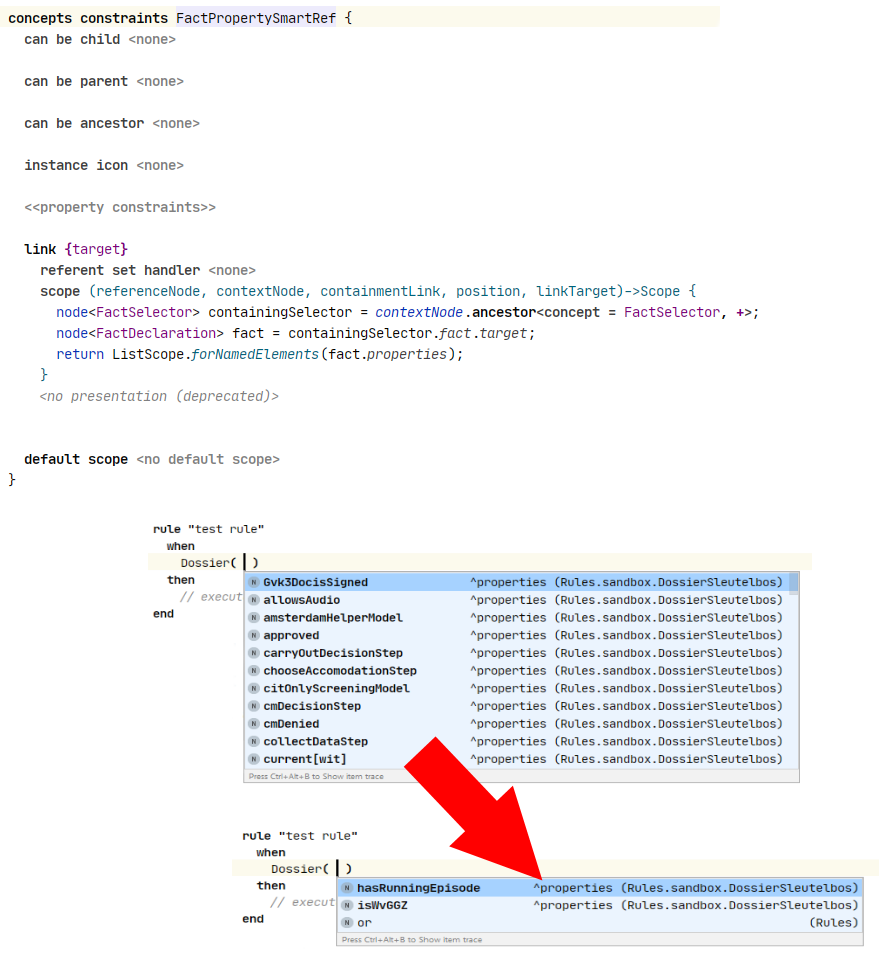
\includegraphics[width=0.95\textwidth]{Sections/images/RSRConstraint.png}}
    \caption{RSR Scoping Constraint}
    \label{fig:RSRConstraint}
\end{figure}

Thus, we have described the entire implementation of the Really Simple Rules Language.

After implementing the language we wrote a program with a large number of rules.
This program on which we will experiment with the different projections.
An example of our default Drools like text projection is show in figure \ref{fig:RSRProgram}.

\begin{figure}[h]
    \centering
    \fbox{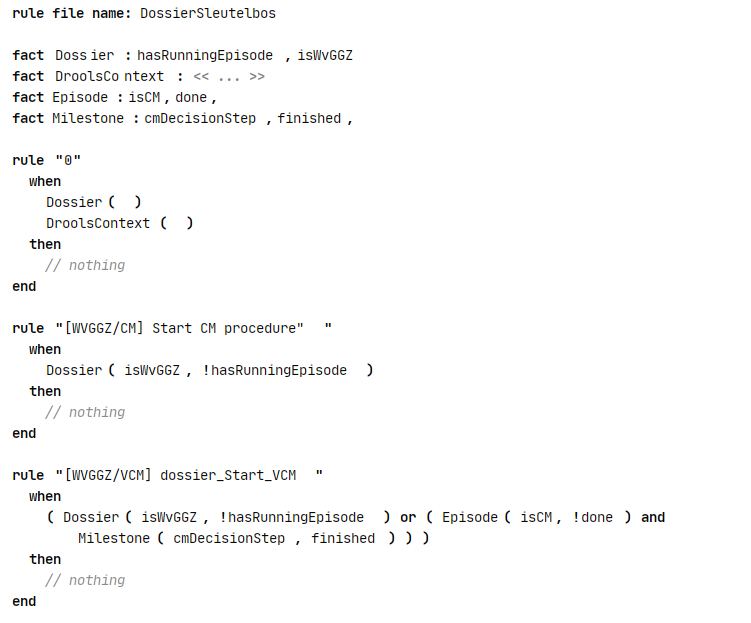
\includegraphics[width=0.95\textwidth]{Sections/images/RSRProgram.png}}
    \caption{RSR program}
    \label{fig:RSRProgram}
\end{figure}

The alternative projections will be discussed in the results section \ref{section:Results_ADR}.

\subsection{Drools-Lite Language}

The RSR was useful as an initial language, however is suffered two major Issues.
Firstly, it's limitations as a language were so great that it was not able to handle many necessary scenarios.
Secondly, our projections would have to be validated by developers with Drools experience.
For this reason we needed to create a projectional language that was much closer to the Drools language.

Our next Language, Drools-Lite, contains many more of the features of Drools.
The preliminary design is shown in figure \ref{fig:DroolsLiteDiagram}.


\begin{figure}[htbp]
    \centering
    \fbox{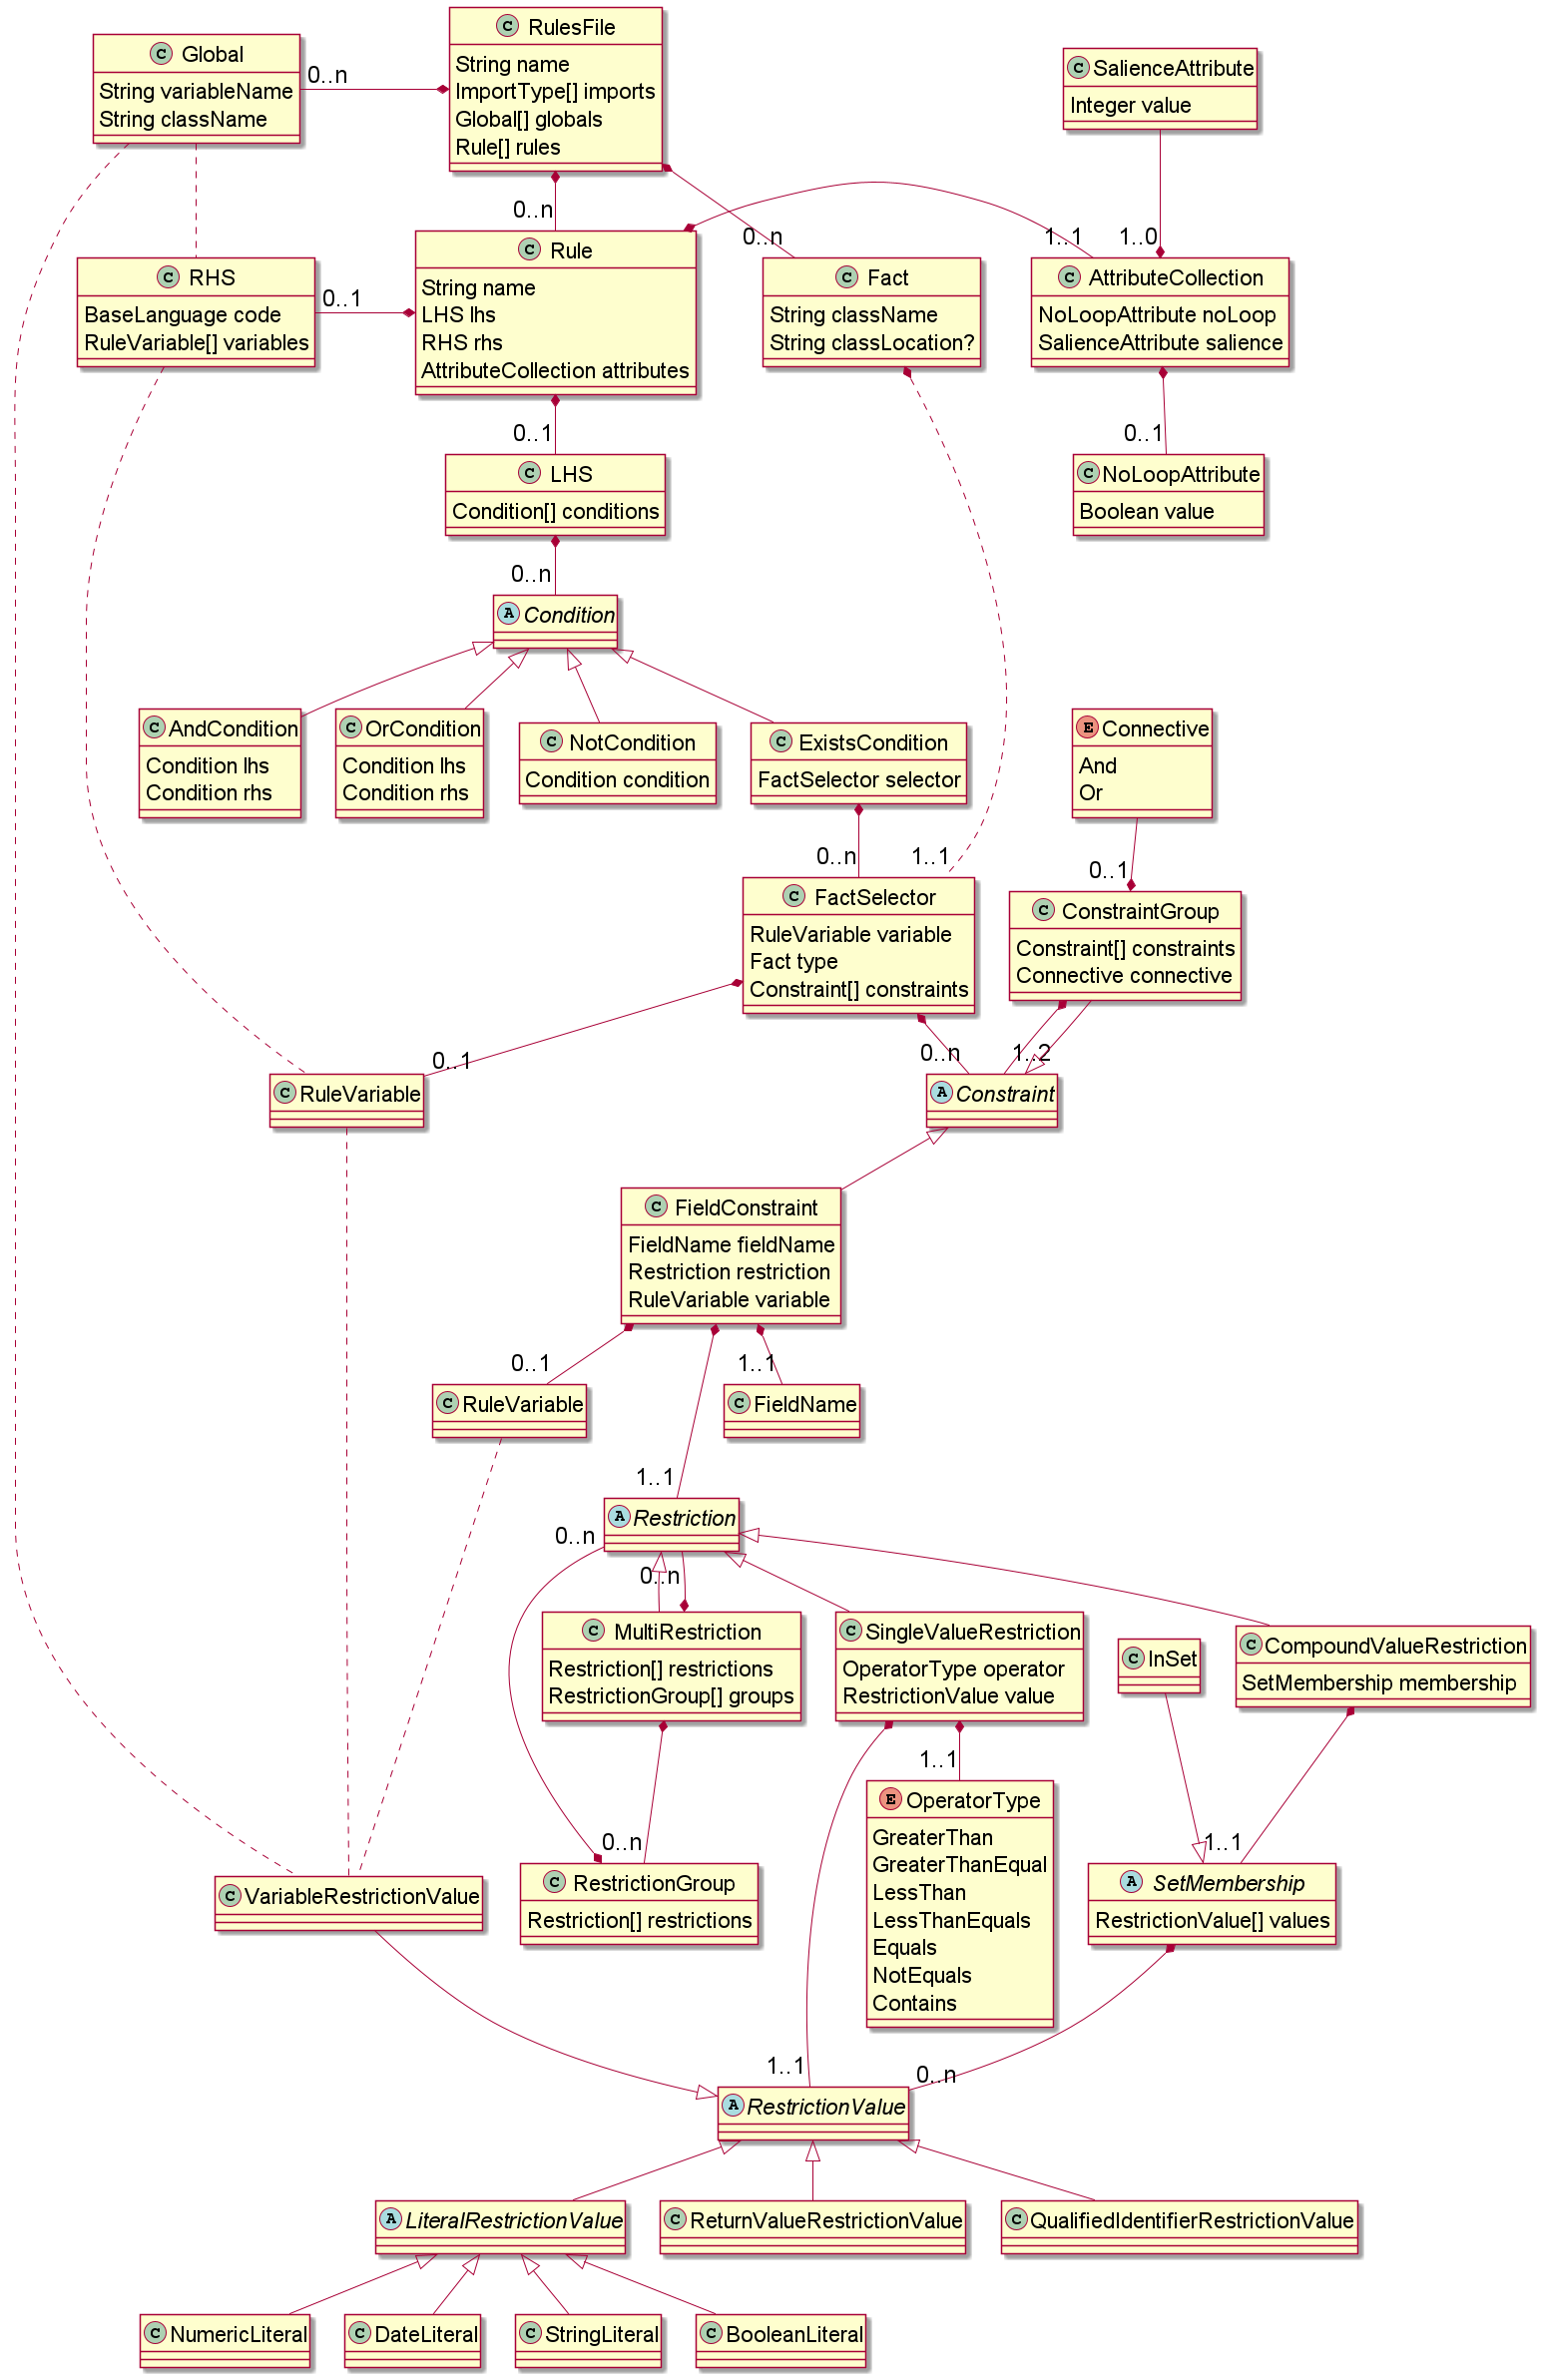
\includegraphics[width=0.85\textwidth]{Sections/images/DroolsLiteStructure.png}}
    \caption{Drools Lite Structure}
    \label{fig:DroolsLiteDiagram}
\end{figure}